\section{Analyse}
\subsection{Hvordan måler vi hældning?}
Før vi kunne begynde på at lave en hældningssensor blev vi nødt til at finde ud af hvilke muligheder der var hældningsumåling. En af mulighederne var at anvende et pendul eller en libelle. Vi startede med at udvikle på en prototype af en libellesensor vist på \textit{Figur~\ref{fig:libelle}}.
\begin{figure}[hbpt]
\centering
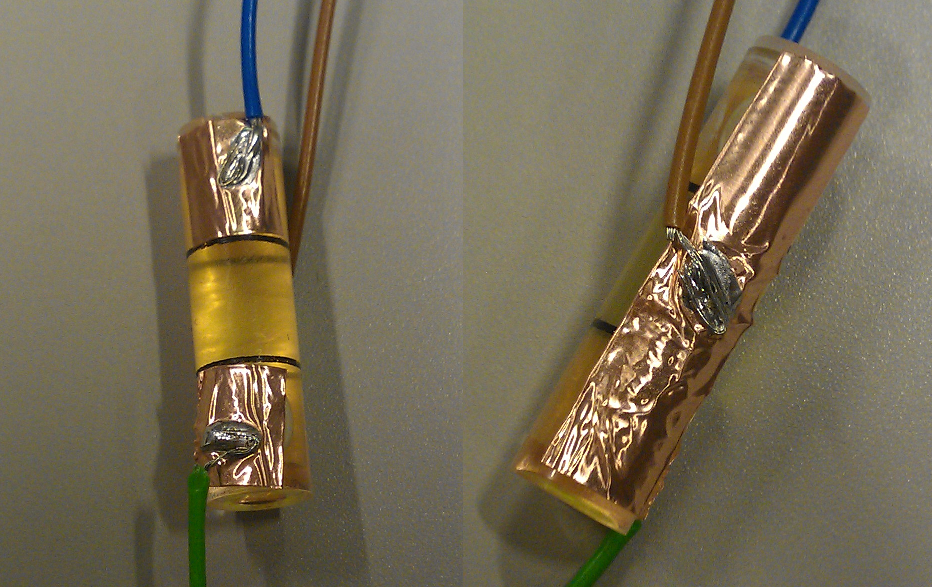
\includegraphics[width=0.4\textwidth]{billeder/libellesensor1}
\caption{Hældningssensor baseret på libelle}
\label{fig:libelle}
\end{figure}
Hældningssensorprototype 1 indeholder 2 højpas filtrer samt en frekvensgenerator og en differensforstærker. Vi kom frem til at libellesensoren har en capacitet på omkring $1*10^{-15}[F]$. Det gør det praktisk umuligt at anvende da vores komponenter i det filter der skulle designes til den færdige sensor, da cutoff frekvens kommer til at være $>3.0[MHz]$. Den høje frekvens giver en stor selvinduktion i vores ledning. Et lavt signal fra hældningssensoren kombineret med stor selvinduktion, gjorde at vi måtte finde en anden løsning.\\
Næste prototype bestod af et potmeter og et pendul. Dog havde potmeteret en for stor friktionsmodstand, der gjorde det upræcist i forhold til vores krav.\\
Vi har gennem et tredje semestersfag fundet ud af at PSoC'en indeholder et accelerometer\footnote{KXSC7-2050 se bilag}. Efter en prototypeopbygning fandt vi ud af at det komponentet opfyldte de krav stille i kravspecifikation. Dog er prototypen implementeret med en '\#define' da databladet er vagt og output varierer mellem PSoCs.
%%%%%%%%%%%%%%%%%%%%
%%% VBTE tis %%%%%%%
%%%%%%%%%%%%%%%%%%%%
\subsubsection{Hvordan måler vi niveauet i vandballasttankene?}
Ultralydsafstandsmålingen blev valgt for at prøve noget ingen havde kendskab til i projektet. Man kunne have valgt at købe en færdiglavet enhed men det blev vurderet at dette ikke gav ret meget faglig erfaring. I e-lab havde de nogle rå tranducere og receivere liggende og der blev derfor valgt at forsøge med at udvikle en ultralydsafstandsmåler. Der blev i starten lavet en del teknologiundersøgelse inden for ultralyden og vi testede tranducere og receivere for at se hvordan de aggerede. Vi fandt at der var en del destruktive reflektioner og vi overvejede at fylde akustisk skum i toppen af tankene, men da det skum vi kunne finde var elektrisk ledende kunne det ikke anvendes. Herudover blev der lavet forsøg med forskellige ultralydskredse fundet på nettet, hvilket gav anledning til erfaring og viden. Jeg kom frem til at et burst skulle sendes for at måle afstanden og en puls på 250$\mu$s blev valgt, hvilket svarer til 10 perioder. Receiverkredsen blev udviklet med viden fra MSE kurset fra sidste semester omkring mixere og operationsforstærkere.

%%%%%%%%%%%%%%%%%%%%
%%% forsyning %%%%%%
%%%%%%%%%%%%%%%%%%%%
\subsection{Hvordan skal de forskellige modulerne forsynes?}
Da modulerne sidder rundt om i skibbet, skal der overvejes hvordan de kan forsynes. Dette kan ske på flere forskellige måder:
\begin{itemize}
\item Batteri
	\begin{itemize}
	\item Smart da man ungår at trække en ledning med forsyning.
	\item Dette kan være meget problematisk med et batteri, da der ikke vides hvor meget strøm der skal trækkes dvs. stort det skal være. 
	\item Da der i forvejen er en kablet kommunikation, skal der alligevel kabel ud til modulet, derfor kan det være lige så smart at have en kablet forsyning.
	\end{itemize}
\item Kablet forsyning \\
Ved at vælge at bruge en kablet forsyning dukker der andre spørgsmål op.
\begin{itemize}
\item F.eks. hvilken forsyningsspænding skal der være.?\\
24V, 230V, 12V, 5V eller noget helt andet..
\end{itemize}
Da der ikke er 100\% kendskab til hvilke forsyning spænding der er på et skib, men nok er 230V AC skal der med stor stor sandsynlighed bruges en strømforsyning til modulerne, da de bruger en lavere spænding. \\
Ved at have en transformator kan spænding evt. komme ned på 24V AC. De 24V AC kan føres ud til modulerne samme med kommunikationen. \\
Ved modulerne kan der bygges en strømforsyning der regulere de 24V AC om til DC. \\
Her kommer der to muliglige strømforsyninger op:
\begin{itemize}
\item En SMPS: \textit{Effektiv, høj virkningsgrad.}
\item En lineær strømforsyning: \textit{Stabil, mellem virkningsgrad}
\end{itemize}
Da virkningsgraden ikke har stor bestydning for produktet, samt erfaringen med SMPS ikke er stor, vil der tages udgangspunkt i en lineær størmforysning.
\end{itemize}
Ved udviklingen af prototypen, kan der overvejes om der skal designes en eller flere strømforsyninger.


%%%%%%%%%%%%%%%%%%%%
%%Kontrolinterface%%
%%%%%%%%%%%%%%%%%%%%

\subsection{Raspberry Pi som host for Kontrolinterfacet}
I den indledende fase var det gruppens ønske at kunne implementere Kontrolinterfacet på et Raspberry Pi-modul. Denne mulighed blev undersøgt, og det viste sig at det godt kunne lade sig gøre at skrive Qt-programmer til Raspberry Pi'en hvis man anvendte den nyeste beta-version af Qt.\\
Versionerne imellem var der dog store forskelle på fundamentale områder af frameworket; nogle af teknologiundersøgelserne måtte derfor undersøges igen.\\
Det var også oprindeligt gruppens ønske at anvende I2C-protokollen mellem Kontrolinterfacet og Styringsmodulet. Denne protokol er også understøttet af Raspberry Pi, men kan kun implementeres med Python medmindre der selv udvikles kernemoduler.\\
Dette var en større opgave end gruppen ønskede at prioritere den. Vi begyndte derfor at kigge efter andre protokoller.\\
Næste emne var rs232-protokollen, da den er kendt for gruppen. Protokollen viste sig at være god med Raspberry Pi. Efter nogle teknologiundersøgelser fandt gruppen også ud af hvordan rs232-kommunikationen kunne implementeres med den nye Qt-version.
Desværre løb gruppen igen i problemer da der skulle kompiles til modulet. Her valgte gruppen at nedprioritere ønsket om at implementere Kontrolinterfacet på Raspberry Pi-modulet og dermed stoppede undersøgelserne.

%%%%%%%%%%%%%%%%%%%%
%%% Databasen %%%%%%
%%%%%%%%%%%%%%%%%%%%
\subsection{Server}
Opbygningen af serveren er gjort på baggrund af behovet for at kunne overføre data via et netværk. Til denne overførelse er TCP blevet valgt grundet erfaring med denne. Ved at benytte TCP, kan der være flere end en der koble til samtidig. TCP giver stabilitet og ordnet levering noget der blev prioriteret højt i prototypen da det er en sikkerhed under lastning og losning. Dette vil sige at hvis en pakke går tabt under overførelsen vil denne automatisk blive forsøgt sendt igen og så er vi sikre på at data kommer frem i samme orden som de blev afsendt. 
Ved TCP kom den udfordring at ved afsendelse fra KI kom alle data over i en streng selv om vi forsøgte at sende dem over i 5 forskellige strenge og satte delays. Dette skyldes at TCP ser det som en streng der skal overføres og ikke som 5. For at løse dette satte vi nul terminering på ved afsendelse. Ved modtagelse blev dataet lagt ind i en variable som blev splittet ved nul terminaringen og efterfølgende gemt. Fra startr var dte meningen at Serveren skulle gemme data direkte til MySQL databasen men grundet problemer med at kompile MySQL header og driver med blev dette efter noget tid droppet og i stedet blev backup muligheden der også er indskravet i kravspecifiklationen ophøjet til eneste mulighed.

\subsection{Valg af database}
For at vælge database til systemet blev der kigge på MySQL, Microsoft Acces og en lagring til en tekstfil.\\
Microsoft Acces er et database system der medfølgende i Microsoft Office pakken. Microsoft Access benytter sit eget format baseret på Access Jet Database Engine. En ulempe ved Microsoft Acces er at den kun fungere under Windows og da systemet skulle være alsidigt var dette ikke den bedste løsning. At lagre direkte i en tekst fil blev overvejet da det er meget simpelt at lagre til tekstfiler fra c++ og php kan håndtere at hente fra den. Det kan gå galt ved loading og lagring til filen samtidig med at formater kan blive et problem. \\
Der var i forvejen kendskab til MySQL og dette er et færdig udviklet system til at fungere med webinterfaces og for programmerings sprog som C++ er der udviklet header. Systemet er et system der fungere på mange platforme og løbende bliver udviklet på. På baggrund af dette blev dette system valgt.

\subsection{Webinterface}
Til den grafiske brugere grænseflade for Databasen blev et Webinterface valgt på baggrund af muligheden for at flere på havneterminalen kunne tilgå dataerne på samme tid. På baggrung af et på forhånd middel kendskab til php som er et  intepretere sprog og dens intergrationen med MySQL database blev php valgt som sprog til kodning af Webinterfacet. Php giver desuden mulighed for at benytte ajax princippet og at bygge en hoved side der includere de andre sider. Dette giver mulighed for at let veligeholdes samt minimal dataoverførelse fra webserveren som m indsker loarding time.

%%%%%%%%%%%%%%%%%%%%
%%% Jura %%%%%%
%%%%%%%%%%%%%%%%%%%%
\subsection{Jura}
I dette afsnit vil vi beskrive de vigtigste juridiske problem stillinger som vi har arbejdet ud fra.

I startfasen blev de forskellige juridiske problemstillinger undersøgt. Dette gav grund til en del overvejelser omkring opbygningen systemet BROS. Ansvars havene personer samt krav til ballastvand er blevet overvejet. Et udplik af de vigtigste begraber findes i bilag for Jura.
Til uddybelse af disse problemstillinger er Maersk blevet kontaktet, desværre har vi ikke fået noget svar. De uridske problemstillinger har bl.a. gjort at projektet blev indskrænket til kun at omhandle bulk skibe samt skibe i nationalt farvand.

